\documentclass[11pt, a4paper, titlepage, openright]{article}

\usepackage[a4paper, total={6.5in, 9.5in}]{geometry}
\usepackage{amssymb}
\usepackage{amsmath}
\usepackage[bottom]{footmisc}
\usepackage{color}
\usepackage{eurosym}
\usepackage{epstopdf}
\usepackage{fixltx2e}
\usepackage{float}
\usepackage[font=small,labelfont=bf]{caption}
\usepackage{graphicx}
\usepackage{hyperref}
\usepackage{listings}
\usepackage{lscape}
\usepackage{mathtools}
\usepackage{rotating}
\usepackage[titletoc, title]{appendix}
\usepackage{wrapfig}

\usepackage{matlab-prettifier}
\usepackage{mathtools,booktabs}
\DeclarePairedDelimiter\ceil{\lceil}{\rceil}
\DeclarePairedDelimiter\floor{\lfloor}{\rfloor}

\restylefloat{figure}
\setlength\parindent{0pt}

\lstset{
    frame=tb,
    aboveskip=3mm,
    belowskip=3mm,
    showstringspaces=false,
    basicstyle={\footnotesize\ttfamily},
    numbers=none,
    breaklines=true,
    breakatwhitespace=true,
    tabsize=4,
    showstringspaces=false,
    keepspaces=true,
    columns=fullflexible
}

\newenvironment{verbquote}
	{\catcode `^=12% Math superscript
	\catcode `_=12% Math subscript
	\catcode `$=12% Math deliniation
	\begin{quote}}
	{\end{quote}}

\begin{document}
%%%%%%%%%%%%%%%%%%%%%%%%%%%%%%%%%%%%%%%%%
% University Assignment Title Page
% LaTeX Template
% Version 1.0 (27/12/12)
%
% This template has been downloaded from:
% http://www.LaTeXTemplates.com
%
% Original author:
% WikiBooks (http://en.wikibooks.org/wiki/LaTeX/Title_Creation)
%
% License:
% CC BY-NC-SA 3.0 (http://creativecommons.org/licenses/by-nc-sa/3.0/)
%
% Instructions for using this template:
% This title page is capable of being compiled as is. This is not useful for
% including it in another document. To do this, you have two options:
%
% 1) Copy/paste everything between \begin{document} and \end{document}
% starting at \begin{titlepage} and paste this into another LaTeX file where you
% want your title page.
% OR
% 2) Remove everything outside the \begin{titlepage} and \end{titlepage} and
% move this file to the same directory as the LaTeX file you wish to add it to.
% Then add \input{./title_page_1.tex} to your LaTeX file where you want your
% title page.
%
%%%%%%%%%%%%%%%%%%%%%%%%%%%%%%%%%%%%%%%%%

%----------------------------------------------------------------------------------------
%	PACKAGES AND OTHER DOCUMENT CONFIGURATIONS
%----------------------------------------------------------------------------------------
\begin{titlepage}

\newcommand{\HRule}{\rule{\linewidth}{0.5mm}} % Defines a new command for the horizontal lines, change thickness here

\center % Center everything on the page

%----------------------------------------------------------------------------------------
%	HEADING SECTIONS
%----------------------------------------------------------------------------------------

\textsc{\LARGE KU Leuven}\\[1.5cm] % Name of your university/college
\textsc{\Large }\\[4cm] % Major heading such as course name
\textsc{\Large Modellering en simulatie}\\[0.5cm] % Minor heading such as course title

%----------------------------------------------------------------------------------------
%	TITLE SECTION
%----------------------------------------------------------------------------------------

\HRule
{ \huge \bfseries Practicum 1:\\ \Large{Monte Carlo-simulaties}}\\ % Title of your document
\HRule \\[1.5cm]

%----------------------------------------------------------------------------------------
%	AUTHOR SECTION
%----------------------------------------------------------------------------------------

\begin{minipage}{0.4\textwidth}
\begin{flushleft} \large
Armin Halilovic - r0679689 % Your name
\end{flushleft}
\end{minipage}
~
\begin{minipage}{0.4\textwidth}
\begin{flushright} \large
\end{flushright}
\end{minipage}\\[4cm]

% If you don't want a supervisor, uncomment the two lines below and remove the section above
%\Large \emph{Author:}\\
%John \textsc{Smith}\\[3cm] % Your name

%----------------------------------------------------------------------------------------
%	DATE SECTION
%----------------------------------------------------------------------------------------

\vfill % Fill the rest of the page with whitespace
{\large 2 December 2016}\\[3cm] % Date, change the \today to a set date if you want to be precise

%----------------------------------------------------------------------------------------
%	LOGO SECTION
%----------------------------------------------------------------------------------------

%\includegraphics{Logo}\\[1cm] % Include a department/university logo - this will require the graphicx package

%----------------------------------------------------------------------------------------


\end{titlepage}
\tableofcontents
\newpage

In dit verslag worden oplossingen gegeven voor de opdrachten in het practicum.
De code voor alle opdrachten staat onder appendix A.

\section{Een aanbevelingssysteem voor films}
	\subsection{Matrixvervollediging}

	\subsubsection{Opdracht 2}
	\begin{quote}
        Hoeveel geheugenruimte is nodig om de volle beoordelingenmatrix full(R) voor te stellen? \\
        Hoeveel geheugenruimte is nodig om de ijle beoordelingenmatrix R voor te stellen in het coordinaatformaat? \\
        Hoeveel geheugenruimte is vereist om de rang-r lagerangbenadering \( W F^T \) uit verg. (2) compact voor te stellen (als functie van r)? \\
        Maak een duidelijke figuur waarin je het geheugengebruik van de lagerangbenadering uit verg. (2) en het
        geheugengebruik van de ijle matrix R uitzet als functie van r voor de waarden \( r = 1, ..., 500 \) \\
        Voor welke waarde van r snijden deze twee lineaire functies?
	\end{quote}

    Om de volle beoordelingenmatrix full(R) (\( R \in \mathbb{R}^{m \times n} \)) voor te stellen
    is er \( 8 \times m \times n \) bytes geheugenruimte nodig. \\

    Om een matrix in coordinaatformaat op te slaan zijn verzamelingen van rij-indices \(i\),
    kolom-indices \(j\), en waarden \( r_{i,j} \) nodig. De verzamelingen van indices kunnen bestaan
    uit gehele getallen. Er is dus \[ 4 \times r + 4 \times r + 8 \times r = 16 \times r \] bytes
    geheugenruimte nodig voor het coordinaatformaat, waarbij r het aantal niet-nulwaarden is van \( R\). \\

    Om de rang-r lagerangbenadering \( R \approx WF^T (W \in \mathbb{R}^{m \times r}, F \in \mathbb{R}^{n \times r} ) \)
    voor te stellen is er  \[ 8 \times m \times r + 8 \times n \times r = 8r (m + n) \]  bytes geheugenruimte nodig.

	\begin{figure}[H]
		\centering
		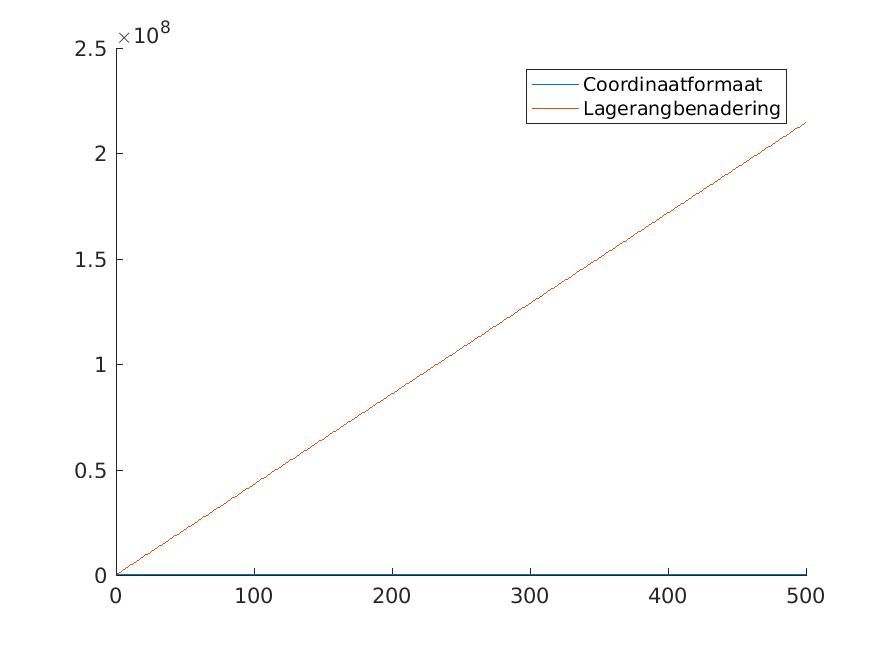
\includegraphics[width=0.7\linewidth]{../ex2}
		\caption{Het geheugengebruik van de lagerangbenadering en van de beoordelingenmatrix in coordinaatformaat}
		\label{fig:ex2}
	\end{figure}

    TODO: De twee functies snijden nooit en ik moet de berekening eens checken.

	\subsubsection{Opdracht 3}
    \begin{quote}
        Bewijs dat \(\sigma_j\) de \(j^de\) grootste singuliere waarde van A is en dat
        \[ A - E_k = \sum\limits_{j=1}^{k} \sigma_j \textbf{u}_j \textbf{v}_j^T \]
        de rang-k (met \( k \leq r \)) afgeknotte singulierewaardeontbinding van A is.
    \end{quote}

    TODO: Bewijs eens uitschrijven.

	\subsubsection{Opdracht 4}
    \begin{quote}
        Stel dat we de stappen 4–6 van algoritme 1 slechts eenmaal zouden uitvoeren.
        Kan men dit algoritme dan toepassen op een 240 000 x 33 000 matrix met 22 miljoen niet-nulwaarden
        (i.e., de volledige MovieLens databank) op een laptop met 8GB werkgeheugen en 32GB swap geheugen? Waarom wel of niet?
    \end{quote}

    Dit is mogelijk als ijle matrices worden gebruikt en als het ijlhijdspatroon kan worden behouden.
    Bij gebruik van volle matrices is er te veel geheugenruimte nodig.

	Output van de code (zie \ref{appendix:ex4}):
\begin{lstlisting}
Totaal bruikbaar geheugen: 40GB
Nodig geheugen met volle matrices: 190.08GB
Nodig geheugen als het ijlhijdspatroon behouden kan worden: 1.06GB
\end{lstlisting}

	\subsubsection{Opdracht 5}
    \begin{quote}
        function [X] = SN\_sparseModel(Uk, sk, Vk, A) \\
        De geheugencomplexiteit van je algoritme in functie van m, n, r en \(\zeta\) mag hoogstens \(\mathcal{O}(\zeta)\) bedragen
        - je mag hierbij wel veronderstellen dat \( max\{m, n\} \leq \zeta \). Hoe heb je deze doelstelling bereikt?
    \end{quote}

    Zie \ref{appendix:sparseModel}. \\
    De doelstelling werd bereikt door enkel plaats te alloceren voor vectoren met lengte \( \zeta \):
\begin{lstlisting}[style=Matlab-editor, basicstyle = \scriptsize]
[i, j, v] = find(A);
\end{lstlisting}
     \(i\), \(j\), en \(v\) zijn vectoren
    die de matrix A voorstellen in coordinaatformaat. De waarden in vector v worden dan overschreven door de waarden die horen te staan in
    \( U_k * diag(s_k) * V_k^T \) op dezelfde posities (\(i, j\)):
\begin{lstlisting}[style=Matlab-editor, basicstyle = \scriptsize]
for val = 1:length(i)
    v(val) = Uk(i(val), :) .* sk' * Vk(j(val), :)';
end
\end{lstlisting}
    Deze nieuwe waarden worden een per een berekend, aangezien een uitgewerkte kopie van
    \( U_k * diag(s_k) * V_k^T \) bijhouden geheugencomplexiteit \(\mathcal{O}(m*n)\) zou bedragens.

	\subsubsection{Opdracht 6}
    \begin{quote}
        function [s] = SN\_optimalCoefficients(Uk, Vk, A) \\
        De geheugencomplexiteit van je algoritme in functie van m, n, k en ζ mag hoogstens \(\mathcal{O}(k\zeta)\) bedragen
        - je mag hierbij wel veronderstellen dat \( max\{m, n\} \leq \zeta \). Hoe heb je deze doelstelling bereikt?
    \end{quote}

    Zie \ref{appendix:optimalCoefficients}. \\
    De doelstelling werd bereikt door plaats te alloceren voor \(k\zeta\) elementen voor de matrix B:
\begin{lstlisting}[style=Matlab-editor, basicstyle = \scriptsize]
B = sparse([], [], [], m*n, k, nnz(A) * k);
\end{lstlisting}
    Tijdens het invullen van deze matrix werd enkel gebruik gemaakt van de sparseModel functie,
    die geheugencomplexiteit \(\mathcal{O}(\zeta)\) bedraagt.

	\subsubsection{Opdracht 8}
    \begin{quote}
        Hoeveel bedragen de 3 laagste gemiddelde beoordelingen? Hoeveel gebruikers gaven exact 5 als gemiddelde score?
    \end{quote}

	Output van de code (zie \ref{appendix:ex8}):
\begin{lstlisting}
De drie laagste gemiddelde beoordelingen zijn:
	 0.81 van gebruiker 40142
	 0.98 van gebruiker 33685
	 1.04 van gebruiker 10405
39 gebruikers hebben een gemiddelde score van exact 5.
\end{lstlisting}

	\subsubsection{Opdracht 10}
    \begin{quote}
        Hoeveel bedraagt de RMSE tussen T en de ijle matrix \( P_{\Omega}(\boldsymbol{\mu} \boldsymbol{1}^T ) \)?
    \end{quote}

	Output van de code (zie \ref{appendix:ex10}):
\begin{lstlisting}
RMSE tussen T en de ijle matrix: 0.905725
\end{lstlisting}

	\subsubsection{Opdracht 11}
    \begin{quote}
        Pas SN\_rank1MatrixPursuit toe op de gekende beoordelingenmatrix R, waarbij je r = 30 als gewenste rang kiest en de testdata T
        als derde argument kiest. Maak een duidelijke figuur van de evolutie van de RMSE.
    \end{quote}

    \begin{figure}[H]
        \centering
        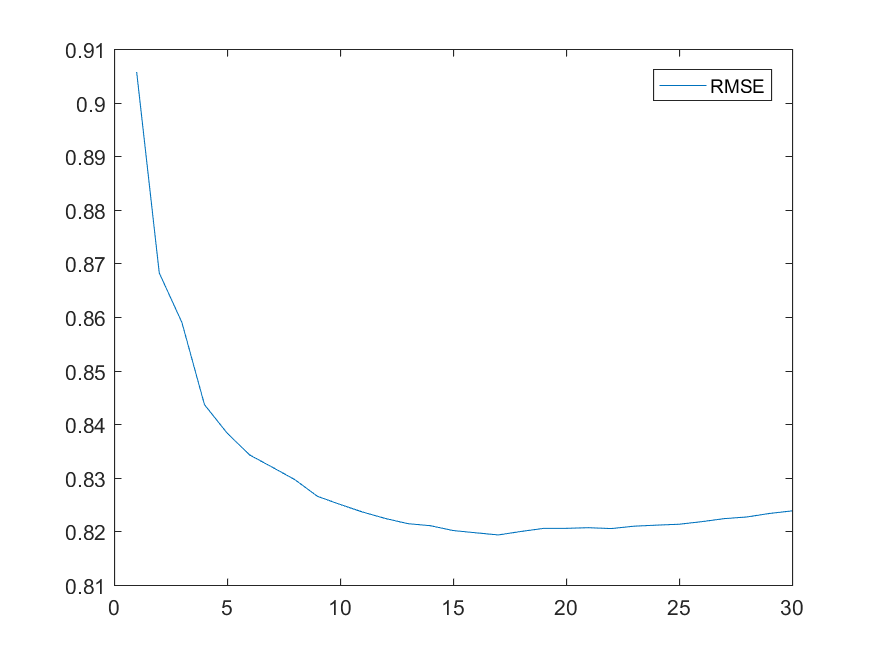
\includegraphics[width=0.7\linewidth]{../ex11}
        \caption{De evolutie van de RMSE bij toepassing van rank1MatrixPursuit(R, 30, T)}
        \label{fig:ex2}
    \end{figure}

	\subsubsection{Opdracht 12}
    \begin{quote}
        Bereken [U20, s20, V20, $\sim$] = SN\_rank1MatrixPursuit(R, 20, T). Wat zijn de waarden van de vector s20, afgerond tot 2 cijfers na de komma?
    \end{quote}

	Output van de code (zie \ref{appendix:ex12}):
\begin{lstlisting}
   0.97
1584.82
 754.94
 740.23
 572.71
 471.93
 330.87
 334.54
 255.20
 300.50
 281.20
 265.00
 201.74
 208.67
 235.44
 166.34
 188.72
 184.68
 174.97
 175.14
\end{lstlisting}

	\subsubsection{Opdracht 14}
    \begin{quote}
        function [movieIDs, score] = SN\_predictedBestMovies(Uk, sk, Vk) \\
        De geheugencomplexiteit van je algoritme in functie van m, n en k mag hoogstens \(\mathcal{O}(max\{m, n\})\) bedragen.
        Hoe heb je deze doelstelling bereikt?
    \end{quote}

    Zie \ref{appendix:predictedBestMovies}. \\
    De doelstelling werd bereikt door per film elke beoordeling apart te berekenen en op te tellen in een variabele:
\begin{lstlisting}[style=Matlab-editor, basicstyle = \scriptsize]
tmp = sk .* Vk(movie, :)';
sum = 0;
for rating = 1:m
    sum = sum + Uk(rating, :) * tmp;
end
\end{lstlisting}
    De gemiddelde score per film werd dan berekend en opgeslagen in de output vector \( \boldsymbol{score} \). Het berekenen van een beoordeling
    \( U_k(rating, :) \ .* s_k * V_k(movie, :)^T \) bedraagt geheugencomplexiteit  \(\mathcal{O}(k) < \mathcal{O}(max\{m, n\})\).


	\subsubsection{Opdracht 15}
    \begin{quote}
        Bereken met behulp van de functies uit de twee voorgaande opgaves de 25 films met de hoogste gemiddelde beoordelingen
        (op basis van de gekende beoordelingenmatrix R) en de 25 films met de hoogste gemiddelde voorspelde beoordelingen. \\
        Welke lijst van films vind je het meest realistisch? Motiveer je keuze. Onderzoek in het bijzonder het aantal gekende
        beoordelingen in de trainingsdata R van de films in de twee lijsten en betrek deze informatie in je motivering.
    \end{quote}

	Output van de code (zie \ref{appendix:ex15}):
\begin{lstlisting}
average rating - movie ID - movie name - number of reviews
Processing actualBestMovies...
4.31 -  938 - Band of Brothers (2001)                                                    -  2988
4.29 - 4455 - Death on the Staircase (Soupçons) (2004)                                   -    17
4.24 -  510 - City of God (Cidade de Deus) (2002)                                        -  9687
4.23 - 1750 - Lives of Others, The (Das leben der Anderen) (2006)                        -  4400
4.23 - 2486 - Dark Knight, The (2008)                                                    - 15052
4.20 -  390 - Spirited Away (Sen to Chihiro no kamikakushi) (2001)                       - 10553
4.20 -  183 - Amelie (Fabuleux destin d'Amélie Poulain, Le) (2001)                       - 18057
4.18 - 4418 - Frozen Planet (2011)                                                       -    30
4.18 - 3477 - Inception (2010)                                                           - 10541
4.16 -  822 - Lord of the Rings: The Return of the King, The (2003)                      - 23862
4.15 - 4066 - Intouchables (2011)                                                        -  2136
4.15 -  194 - Lord of the Rings: The Fellowship of the Ring, The (2001)                  - 27243
4.14 - 4158 - Black Mirror (2011)                                                        -   467
4.13 - 4227 - Bleak House (2005)                                                         -    30
4.12 -  483 - Lord of the Rings: The Two Towers, The (2002)                              - 25214
4.11 -  892 - Eternal Sunshine of the Spotless Mind (2004)                               - 17391
4.11 - 1932 - Departed, The (2006)                                                       - 11450
4.10 -  825 - Fog of War: Eleven Lessons from the Life of Robert S. McNamara, The (2003) -  2080
4.10 - 4781 - Whiplash (2014)                                                            -   505
4.09 - 1227 - Old Boy (2003)                                                             -  5161
4.08 - 4549 - Louis C.K.: Oh My God (2013)                                               -   243
4.08 - 3786 - Louis C.K.: Shameless (2007)                                               -   711
4.08 - 4755 - Normal Heart, The (2014)                                                   -    33
4.08 -  942 - Best of Youth, The (La meglio gioventù) (2003)                             -   340
4.07 - 3784 - Louis C.K.: Chewed Up (2008)                                               -   568
Processing rank1MatrixPursui
Processing predictedBestMovies...
4.09 -  183 - Amelie (Fabuleux destin d'Amélie Poulain, Le) (2001)                       - 18057
4.07 -  822 - Lord of the Rings: The Return of the King, The (2003)                      - 23862
4.07 - 2486 - Dark Knight, The (2008)                                                    - 15052
4.06 -  194 - Lord of the Rings: The Fellowship of the Ring, The (2001)                  - 27243
4.04 -  892 - Eternal Sunshine of the Spotless Mind (2004)                               - 17391
4.03 -  483 - Lord of the Rings: The Two Towers, The (2002)                              - 25214
4.00 -  510 - City of God (Cidade de Deus) (2002)                                        -  9687
3.99 -  390 - Spirited Away (Sen to Chihiro no kamikakushi) (2001)                       - 10553
3.97 - 1932 - Departed, The (2006)                                                       - 11450
3.95 - 3477 - Inception (2010)                                                           - 10541
3.92 -  154 - Donnie Darko (2001)                                                        - 14884
3.91 - 1456 - Batman Begins (2005)                                                       - 15237
3.90 -  497 - Pianist, The (2002)                                                        -  8414
3.90 - 1928 - Pan's Labyrinth (Laberinto del fauno, El) (2006)                           -  9356
3.90 -  196 - Beautiful Mind, A (2001)                                                   - 17031
3.90 - 2586 - WALL·E (2008)                                                              -  9987
3.90 - 1955 - Prestige, The (2006)                                                       -  9379
3.88 -  761 - Kill Bill: Vol. 1 (2003)                                                   - 17613
3.87 -  625 - Finding Nemo (2003)                                                        - 18674
3.87 - 2336 - No Country for Old Men (2007)                                              -  8489
3.86 - 1109 - Incredibles, The (2004)                                                    - 15972
3.86 -  310 - Bourne Identity, The (2002)                                                - 16295
3.86 - 1738 - V for Vendetta (2006)                                                      - 11978
3.85 -  652 - Pirates of the Caribbean: The Curse of the Black Pearl (2003)              - 20025
3.85 - 2944 - Inglourious Basterds (2009)                                                -  7805
\end{lstlisting}

    De tweede lijst van films vind ik het meest realistisch. Wat hier meteen opvalt is dat de films met weinig beoordelingen
    uit de top zijn verdewenen (in dit geval, alle films met minder dan 5162 beoordelingen). Deze films hadden weinig beoordelingen,
    maar alle beoordelingen waren hoog genoeg om de films in de top 25 te doen belanden. Een film met 1 beoordeling van 5 zal bijvoorbeeld
    als eerste in de lijst staan. \\
    De lijst die uit predictedBestMovies komt werkt dit effect tegen. Het aantal beoordelingen per flim speelt hier ook een
    belangrijke factor in het bepalen van de score. Om nu in de lijst te belanden, moet een film een relatief hoog aantal beoordelingen hebben
    met een hoge waarde. \\

    Daarnaast valt ook op dat de Lord of the Rings films en The Dark Knight hoger in de lijst staan en dat Batman Begins en The Prestige
    nieuw in de lijst een vrij hoge plaatsen hebben gekregen, wat de tweede lijst duidelijk een betere keuze maakt.
	\subsection{Clustering}

	\subsubsection{Opdracht 16}
    \begin{quote}
        function [C] = SN\_correlationMatrix(Uk, sk, Vk) \\
        De geheugencomplexiteit van je algoritme in functie van m, n en k mag hoogstens \(\mathcal{O}(k^2 + n^2)\) bedragen.
        Hoe heb je deze doelstelling bereikt?
    \end{quote}

    Zie \ref{appendix:correlationMatrix}. \\
    De doelstelling werd bereikt door de formule voor de correlatiematrix C
    \[ C = \frac{1}{m - 1} ((R_k - \boldsymbol{1}\boldsymbol{\mu}^T) \Sigma^{-1})^T ((R_k - \boldsymbol{1}\boldsymbol{\mu}^T) \Sigma^{-1}) \]
    te herschrijven zodat \( R_k \in \mathbb{R}^{n \times n} \) ipv \( R_k \in \mathbb{R}^{m \times n} \). \\
    De berekening wordt dan
    \[ C = \Bigg(\sum\limits_{j=1}^{\floor{m/n}} (R_j - \boldsymbol{1}\boldsymbol{\mu}^T)^T * (R_j - \boldsymbol{1}\boldsymbol{\mu}^T)\Bigg) \ ./ \ (\boldsymbol{\sigma} \ .* \boldsymbol{\sigma}^T) \ / \ (m - 1) \]
    waarbij \( R_j \in \mathbb{R}^{n \times n} \), en waarbij \(\mu \in \mathbb{R}^{n} \) de gemiddeldes en \( \sigma \in \mathbb{R}^{n} \) de standaardafwijkingen bevatten voor de beoordelingen van de films.
    In de code worden de blokken \( R_j - \boldsymbol{1}\boldsymbol{\mu}^T \) berekend met geheugencomplexiteit \(\mathcal{O}(n^2)\):
\begin{lstlisting}[style=Matlab-editor, basicstyle = \scriptsize]
R_j = Uk(row_from:min(row_from+n-1, m), :) * V - means';
C = C + (R_j' * R_j);
\end{lstlisting}
    waarbij \(V\) gelijk is aan \( diag(s_k) * V_k^T \). \(V\) bedraagt geheugencomplexiteit \(\mathcal{O}(kn)\). \\
    Aangezien \( R_j \in \mathbb{R}^{n \times n} \) en \( kn < k^2 + n^2 \) altijd geldt wanneer \( k > 0 \),
    wordt de opgelegde beperking van \(\mathcal{O}(k^2 + n^2)\) niet overschreden.

	\subsubsection{Opdracht 18}
    \begin{quote}
        Welke n films zijn het sterkst positief gecorreleerd met de film met volgnummer k, voor volgende waarden van n en k?
        Zijn deze resultaten realistisch? Motiveer. Zijn er gelijkenissen met de aanbevelingen van andere aanbevelingssystemen,
        zoals bijvoorbeeld IMDB.com, MovieLens, Amazon.com of Netflix?
    \end{quote}

	Output van de code (zie \ref{appendix:ex18}):
\begin{lstlisting}
10 most similar movies for Harry Potter and the Chamber of Secrets (2002) (id 446):
    Harry Potter and the Sorcerer's Stone (a.k.a. Harry Potter and the Philosopher's Stone) (2001)
    Harry Potter and the Goblet of Fire (2005)
    Harry Potter and the Prisoner of Azkaban (2004)
    Harry Potter and the Order of the Phoenix (2007)
    Harry Potter and the Half-Blood Prince (2009)
    Chronicles of Narnia: The Lion, the Witch and the Wardrobe, The (2005)
    Harry Potter and the Deathly Hallows: Part 1 (2010)
    Pirates of the Caribbean: Dead Man's Chest (2006)
    Harry Potter and the Deathly Hallows: Part 2 (2011)
    Pirates of the Caribbean: At World's End (2007)

5 most similar movies for Captain America: The First Avenger (2011) (id 3854):
    Thor (2011)
    Amazing Spider-Man, The (2012)
    Iron Man 3 (2013)
    Quantum of Solace (2008)
    Hellboy II: The Golden Army (2008)

3 most similar movies for Zero Dark Thirty (2012) (id 4355):
    Captain Phillips (2013)
    Rush (2013)
    Lincoln (2012)

3 most similar movies for Futurama: Bender's Game (2008) (id 2747):
    Futurama: The Beast with a Billion Backs (2008)
    Fido (2006)
    World's End, The (2013)

9 most similar movies for Monsters, Inc. (2001) (id 160):
    Finding Nemo (2003)
    Incredibles, The (2004)
    Shrek (2001)
    Ratatouille (2007)
    Shrek 2 (2004)
    WALL·E (2008)
    Ice Age (2002)
    Up (2009)
    X2: X-Men United (2003)
\end{lstlisting}

    Deze resultaten lijken mij heel realistisch. De flims die sterk positief correleren met elkaar zijn telkens
    uit dezelfde flim franchises (bv Harry Potter en Futurama met andere Harry Potter en Futurama films),
    flims in hetzelfde genre (Captain America met actie/avonturenfilms, Zero Dark Thirty met actie/drama films, Futurama met komedie flims),
    en films in dezelfde stijl of met detzelfde animatieflim studio's (Monsters, Inc.). \\
    Dit gedrag doet zich ook voor in andere aanbevelingssystemen.

	\subsubsection{Opdracht 19}
    \begin{quote}
        Bewijs dat de correlatiematrix C in de vergelijking
        \[ C = \frac{1}{m - 1} ((R_k - \boldsymbol{1}\boldsymbol{\mu}^T) \Sigma^{-1})^T ((R_k - \boldsymbol{1}\boldsymbol{\mu}^T) \Sigma^{-1}) \]
        hoogstens rang r + 1 heeft wanneer de voorspelde beoordelingenmatrix
        A exact rang r heeft.
    \end{quote}

    TODO: bewijs uitschrijven


\section{Evaluatie}

	\subsection{Opdracht 1}
		\begin{quote}
			Hoeveel tijd heb je gespendeerd aan het oplossen van de opdrachten?
			Hoeveel tijd heb je gespendeerd aan het schrijven van het verslag?
		\end{quote}
        Ik heb ongeveer 25 uur gespendeerd aan het oplossen van de opdrachten en ongeveer 8 uur aan het schrijven van het verslag.

	\subsection{Opdracht 2}
		\begin{quote}
			In de loop van deze opdracht hebben we allerhande veronderstellingen gemaakt om ons nieuw aanbevelingssysteem
            op te stellen. Wat zijn je bedenkingen hierbij? Vind je de resultaten realistisch? Zou je het ontwikkelde
            aanbevelingssysteem durven toevoegen aan de lijst van aanbevelingssystemen van MovieLens?
		\end{quote}
        Op basis van opdrachten 15 en 18 vind ik dat de resultaten van de veronderstellingen realistisch zijn. Aangezien een korte google
        search over aanbevelingssystemen mij een boek van meer dan 500 pagina's aanbeveelt zou ik voor een grote website zoals MovieLens
        niet meteen dit systeem aanbevelen zonder de andere opties eens te bekijken. Er zal waarschijnlijk wel iets efficienter
        of nauwkeuriger zijn. Dit systeem zou misschien wel gebruikt kunnen worden bij mijn studentenjob voor een kleinere website,
        waar een aanbevelingssysteem op de planning staat voor later.

	\subsection{Opdracht 3}
		\begin{quote}
			Welke bedenkingen heb je bij dit practicum? Was de opdracht (veel) te gemakkelijk, (veel) te moeilijk of
			van een gepaste moeilijkheidsgraad? Wat zou je zelf anders aangepakt hebben? Was de terminologie voldoende duidelijk?
		\end{quote}
        Het theoretische aspect van de opdracht is helemaal in orde. Het was een heel interessante toepassing van wat we hebben geleerd.
        Alles in de opdracht was duidelijk. Alles snel genoeg krijgen binnen de opgelegde geheugencomplexiteiten zodat ik niet uren
        zou moeten wachten op resultaten was erg moeilijk. Daar is het meeste van de tijd naartoe gegaan.

\onecolumn
\appendix
\appendixpage
\addappheadtotoc

\section{Functies}

    \subsection{r0679689\_sparseModel.m}
        \lstinputlisting[style=Matlab-editor, basicstyle = \scriptsize]{../r0679689_sparseModel.m}
        \label{appendix:sparseModel}
    \subsection{r0679689\_optimalCoefficients.m}
        \lstinputlisting[style=Matlab-editor, basicstyle = \scriptsize]{../r0679689_optimalCoefficients.m}
        \label{appendix:optimalCoefficients}
    \subsection{r0679689\_userMeans}
        \lstinputlisting[style=Matlab-editor, basicstyle = \scriptsize]{../r0679689_userMeans.m}
    \subsection{r0679689\_RMSE}
        \lstinputlisting[style=Matlab-editor, basicstyle = \scriptsize]{../r0679689_RMSE.m}
    \subsection{r0679689\_rank1MatrixPursuit.m}
        \lstinputlisting[style=Matlab-editor, basicstyle = \scriptsize]{../r0679689_rank1MatrixPursuit.m}
    \subsection{r0679689\_actualBestMovies.m}
        \lstinputlisting[style=Matlab-editor, basicstyle = \scriptsize]{../r0679689_actualBestMovies.m}
    \subsection{r0679689\_predictedBestMovies.m}
        \label{appendix:predictedBestMovies}
        \lstinputlisting[style=Matlab-editor, basicstyle = \scriptsize]{../r0679689_predictedBestMovies.m}
    \subsection{r0679689\_correlationMatrix.m}
        \label{appendix:correlationMatrix}
        \lstinputlisting[style=Matlab-editor, basicstyle = \scriptsize]{../r0679689_correlationMatrix.m}
    \subsection{r0679689\_similarMovies.m}
        \lstinputlisting[style=Matlab-editor, basicstyle = \scriptsize]{../r0679689_similarMovies.m}

\section{Opdrachten}

	\subsection{Opdracht 1}
		\lstinputlisting[style=Matlab-editor, basicstyle = \scriptsize]{../ex1.m}
	\subsection{Opdracht 2}
		\lstinputlisting[style=Matlab-editor, basicstyle = \scriptsize]{../ex2.m}
	\subsection{Opdracht 4}
    \label{appendix:ex4}
		\lstinputlisting[style=Matlab-editor, basicstyle = \scriptsize]{../ex4.m}
    \subsection{Opdracht 5}
        \lstinputlisting[style=Matlab-editor, basicstyle = \scriptsize]{../ex5.m}
    \subsection{Opdracht 6}
        \lstinputlisting[style=Matlab-editor, basicstyle = \scriptsize]{../ex6.m}
    \subsection{Opdracht 8}
        \label{appendix:ex8}
        \lstinputlisting[style=Matlab-editor, basicstyle = \scriptsize]{../ex8.m}
	\subsection{Opdracht 10}
        \label{appendix:ex10}
		\lstinputlisting[style=Matlab-editor, basicstyle = \scriptsize]{../ex10.m}
	\subsection{Opdracht 11}
		\lstinputlisting[style=Matlab-editor, basicstyle = \scriptsize]{../ex11.m}
	\subsection{Opdracht 12}
        \label{appendix:ex12}
		\lstinputlisting[style=Matlab-editor, basicstyle = \scriptsize]{../ex12.m}
	\subsection{Opdracht 15}
        \label{appendix:ex15}
		\lstinputlisting[style=Matlab-editor, basicstyle = \scriptsize]{../ex15.m}
	\subsection{Opdracht 18}
        \label{appendix:ex18}
		\lstinputlisting[style=Matlab-editor, basicstyle = \scriptsize]{../ex18.m}
\end{document}
